
\chapter{Grundlagen}
%Harm
\section{Raspberry Pi}
%TODO: Quellen!
Der Raspberry Pi wurde von der britischen Raspberry Pi Foundation entworfen um
jungen Menschen den Erwerb von Programmier- und Hardwarekenntnissen zu
ermöglichen. Er ist ein Einplatinencomputer und für wenig Geld verfügbar. Der
Raspberry Pi zeichnet sich durch frei programmierbare Schnittstellen aus um
beispielsweise Sensoren anzuschließen.

Mittlerweile gibt es mehrere Modelle:

\begin{itemize} 
\item Pi Zero 
\item Pi Zero W
\item Pi 1 Modell A
\item Pi 1 Modell A+
\item Pi 1 Modell B
\item Pi 1 Modell B+
\item Pi 2 Modell B
\item Pi 3 Modell B 
\end{itemize}

%TODO: Von uns genutzte Modelle hinzufügen
%TODO: Unterschiede der Modelle erläutern

%Jan
\section{Sprachen}

\subsection{Python}\label{Python}
%TODO: Zitierung muss passiv sein
\textsc{Johannes Hubertz}\cite{hubertz2016softwaretests} schreibt, dass Python für alle gängigen Betriebssysteme verfügbar ist und bei Linux-Distributionen wird es direkt mit ausgeliefert. Der Interpreter eignet sich für manuelle Eingaben, die direkt verarbeitet werden. Ebenfalls eignet sich dieser für die Ausführung von Dateien, die Python-Code enthalten. Eine Eigenheit von Python besteht darin, alles als Objekt zu behandeln. Der Quelltext ist durch die besondere Einrückung mit Leerzeichen, der die wesentliche Ausführung bestimmt, einfach und gut lesbar.  Mit der Scriptsprache Python ist es möglich, die Sensoren des Raspberry Pi zu implementieren. Ebenso gibt es die Möglichkeit eine Datenbankschnittstelle zu erstellen und eine Schnittstelle für die Kommunikation unter den Raspberry Pi's.

\subsection{Java}\label{Java}
%TODO: Zitieren im passiv
\textsc{Dietemar Abts} stellt in seinem Buch "'Grundkurs JAVA : von den Grundlagen bis zu Datenbank- und Netzanwendungen"' \cite{abts2015grundkurs} Java als eine universelle Programmiersprache für viele Anwendungen in der Industrie auf Client- und Serverseite dar.
Sie wird als Standard für die Entwicklung von Unternehmenssoftware, Webanwendungen, in technischen Systemen und in mobilen Anwendungen verwendet.
Ein besonderes Merkmal von Java ist die Plattformunabhängigkeit, d.h. Java Anwendungen sind ohne Portierung auf nahezu allen Rechnersystemen 
lauffähig. Java profitiert von den Erfahrungen mit anderen Programmiersprache wie C, C++ und Smalltalk. Wesentliche Konzepte wurden übernommen und fehleranfällige Eigenschaften wurden bewusst ausgelassen, damit die Sprache verhältnismäßig robust und einfach ist.%TODO: Bis hierhin 
Mit der Programmiersprache Java ist es möglich, die Sensoren des Raspberry Pi's zu implementieren. Ebenso können Datenbankschnittstellen und Schnittstellen zur Kommunikation erstellt werden.

\subsection{\ac{SQL}}
%TODO: Zitieren im passiv
Laut \textsc{Edwin Schick}\cite{schicker2017datenbanken} ist \ac{SQL} eine Zugriffsprache für den Endbenutzer. Als Schnittstelle für den Anwender dominieren inzwischen grafische Oberflächen. Für Datenbankprogrammierer hat die Sprache \ac{SQL} an große Bedeutung gewonnen, insbesondere seit der ersten Normierung (SQL1 1987).\ac{SQL} ist die wichtigste Standardsprache für Datenbanken. Die \ac{SQL} Datenbank soll als Speicher für Daten der Raspberry Pi's dienen. Zusätzlich soll die Daten aus der Datenbank lesbar sein.
\subsection{\ac{HTML}}
%TODO: Zitieren im passiv
\textsc{Valentin Plenk}\cite{plenk2017angewandte} schreibt, dass \ac{HTML} eine textbasierte Auszeichnungssprache ist, die von Menschen für Menschen geschrieben Texte strukturiert. Durch den Webbrowser und Gestaltungsvorlagen wie \ac{CSS} wird die visuelle Darstellung der Texte bestimmt. \ac{HTML} kann strukturierte Dokumente durch verschieden Gliederungsebenen, Absätze und Tabellen erstellen. Zusätzlich bietet es Möglichkeiten Hyperlinks, Bilder und andere multimediale Inhalte wiederzugeben. Die Grundlage des World Wide Webs sind \ac{HTML}-Dokumente, die durch die Webbrowser dargestellt werden. Diese Auszeichnungssprache soll zur Darstellung des Projektes im Webbrowser dienen und somit die gesammelten Messdaten u.v.m. anzeigen.

\subsection{\ac{PHP}}
%TODO: Zitieren im passiv
\textsc{Günther Pomaska} schreibt in seinem Buch "'Webseiten-Programmierung Sprachen, Werkzeuge, Entwicklung"' \cite{pomaska2012webseiten-programmierung}, dass \ac{PHP} für die Web-Programmierung entwickelt wurde. Typische Aufgaben von Internetanwendungen werden durch die Sprache abgedeckt, z.B.: Übermittlung von Formulardaten, Anbindung von Datenbanken oder Erzeugen von Webseiten. Gründe für den Einsatz von \ac{PHP} sind, die weite Verbreitung des Open Source-Projekts mit der plattformübergreifenden Anwendung auf unterschiedlichen Betriebssystemen. Der Entwickler profitiert von der Verfügbarkeit von Programmierbausteinen.
%TODO: Transfersatz einbauen

\subsection{JavaScript}
%TODO: Zitieren im passiv
Laut \textsc{Günther Pomaska} \cite{pomaska2012webseiten-programmierung} ist JavaScript nicht mit der objektorientierten Programmiersprache Java in Verbindung zu bringen, obwohl die Syntax der Sprachelemente in vielen Fällen gleich ist. JavaScript ergänzt die Funktionalität von Web-Browsern und ist eine objektbasierte Skriptsprache. Der Browser kann den Inhalt einer Webseite nur statisch abbilden, mit Hilfe von JavaScript können Inhalte dynamisch dargestellt werden. Elemente werden durch Benutzerzugriffe dynamisch verändert, ohne die Seite neu laden zu müssen.
%TODO: Transfersatz einbauen

%Alex
\section{Sensoren}\label{Sensoren_Planung}
Der Raspberry Pi besitzt mit den \ac{GPIO} Pins eine Möglichkeit Sensoren anzusteuern. Nach der Dokumentation der Raspberry Pi Foundation\cite{GPIOMode77:online} können die \ac{GPIO} Pins 3.3V liefern und digitale Signale annehmen. Das neue Raspberry Pi 3 Modell hat den gleichen Aufbau der \ac{GPIO} Pins und die gleiche Pinbelegung. Schematisch wird die \ac{GPIO} Schnittstelle wie folgt dargestellt.
\begin{figure}[h]
	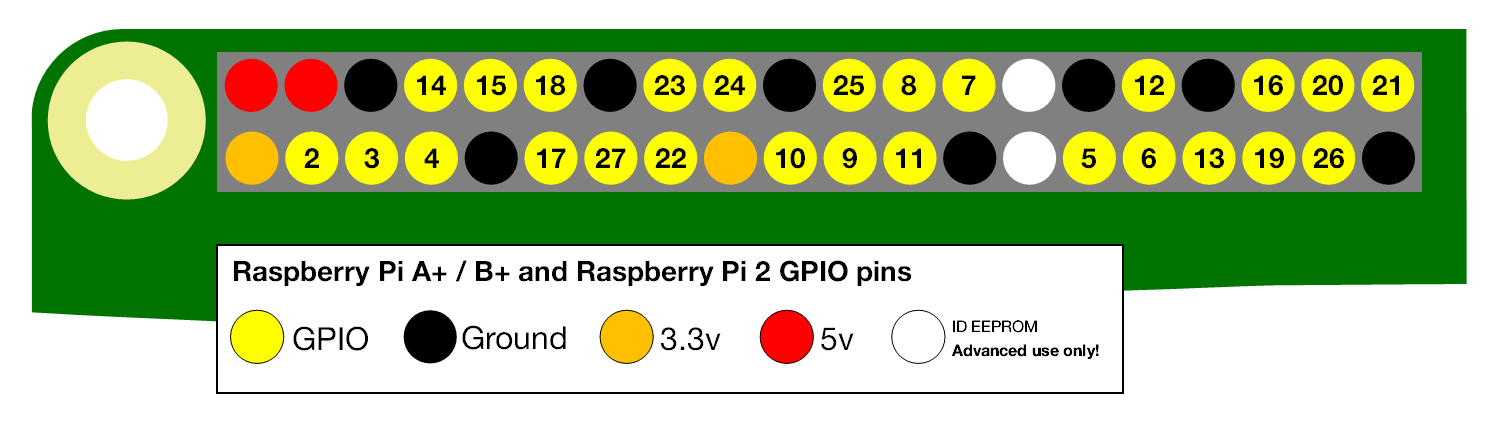
\includegraphics[width=\textwidth]{Bilder/Kapitel2/gpio_pins_pi2.png}
	\caption[Schema GPIO Pins]{Schematische Darstellung der GPIO Pins. Entnommen aus der Raspberry Pi Dokumentation\cite{GPIOMode77:online}.}
	\label{fig:Kapitel2/gpio_pins_pi2.png}
\end{figure}
\noindent
An den vorhandenen 3.3V und 5V Anschlüsse können Sensoren betrieben werden. Dennoch sind nicht alle Sensoren verwendbar. Der Raspberry Pi verfügt nur über die Möglichkeit digitale Signale an den \ac{GPIO} Pins zu verarbeiten. Es werden jedoch neben digitalen auch analoge Sensoren benötigt. Diese können nicht direkt an die Pins angeschlossen werden, aber das Problem wird mit einem \ac{A/D-Wandler} gelöst. \\
Die Erweiterungsplatine RPi-Explorer 700 von Joy-IT \cite{joyitrpi87:online} beinhaltet einen \ac{A/D-Wandler} an dem Analoge Pins angeschlossen werden können. Durch die Erweiterung ist es möglich bis zu vier analoge Sensoren an einem Sensorknoten betrieben werden. \\
Die \ac{GPIO} Schnittstelle unterstützt nur eine maximale Versorgungsspannung von 3.3V, was für die Sensoren ausreichend ist. Durch die Kompatibilität zum Arduino und dem Raspberry Pi können die Sensoren sowohl mit 5V als auch mit 3.3V betrieben werden.
Folgende Sensoren von Allnet\cite{111861pd90:online} werden  im \fullref{Verdrahtung_der_Sensoren} verwendet:
\begin{description}
\item[Temperatur und Luftfeuchtigkeitssensor] \hfill \\
	Der Sensor, KY-015, vom Typ DHT11 kann Temperaturen von 0 bis 50$^\circ$C mit einer Messungenauigkeit von $\pm$ 2$^\circ$C. Die Luftfeuchtigkeit kann im Bereich von 20 bis 95\% ($\pm$ 5\%) gemessen werden. Hierbei handelt es sich um einen digitalen Sensor.  
\item[Flammensensor]\hfill \\
	Der KY-026 besteht aus einer Fotodiode und einem \ac{Poti}. Die Fotodiode kann Wellenlängen im Bereich von etwa 720 - 1100 nm detektieren. Die Diode hat einen Erfassungswinkel von etwa 60$^\circ$. Der \ac{Poti} wird zur Empfindlichkeitseinstellung genutzt, somit kann eine Reichweite von etwa  ein bis sieben Metern abgedeckt werden. Der Sensor besitzt einen "'Digital Out"'-Pin, der high active geschalten wird. Sobald eine Flamme erkannt wird, liegt eine logische 1 auf dem Pin. Der "'Analog Out"'-Pin liefert ein analoges Signal, an welchem bei einer gemessenen Flamme eine niedrige Spannung anliegt.
\item[Lichtschranke]\hfill \\
	Das KY-010 Modul ist eine Lichtschranke, die beim Unterbrechen eine logische 1 an dem digitalen Ausgangspin liefert.
\item[Mikrofon]\hfill \\
	Das Mikrofon, KY-038, hat den gleichen Aufbau wie der Flammensonser. Im Gegensatz zum Flammensensor wird hierbei ein Mikrofonmodul, statt einer Fotodiode genutzt. Die Signale am Digital Out und Analog Out haben die gleiche Funktionalität wie beim Flammensensor. Dieses Modul dient hauptsächlich zur Detektion von kurzen aber lauten Tönen. Ein Anwendungsbeispiel hierfür ist eine Alarmfunktion. Beispielsweise kann das Zerbrechen eines Fensters festgestellt werden.
\item[Lichtsensor]\hfill \\
	Der Lichtsensor KY-018, bestehend aus einem Fotowiderstand, hat bei Dunkelheit einen Widerstand $>$20M$\Omega$ und bei Helligkeit $<$ 80$\Omega$. Damit kann bestimmt werden, ob in einem Zimmer das Licht brennt. Der Lichtsensor liefert ein analoges Signal.
\item[Schocksensor]\hfill \\
	Der Erschütterungssensor liefert eine logische 1 an dem Ausgangspin, falls eine Erschütterung festgestellt wurde. Das dient exemplarisch zur Umsetzung einer Schritterkennung am Boden.
\end{description}

%Harm
\section{WLAN}
\subsection{Standard}
%TODO: "Ich will mehr, viel mehr" - Rammstein
Die Vernetzung erfolgt über ein Funknetz nach dem WLAN-Standard 802.11n. 

\subsection{Verschlüsselung}
%TODO: Einleitung
WEP, WPA, WPA2

Der Vorteil gegenüber der älteren Alternative TKIP ist, dass \ac{CCMP} auf dem AES-Verschlüsselungsstandard basiert. Bei \ac{CCMP} wird ein 128 Bit Schlüssel mit 48 Bit Initialisierungsvektor verwendet.
%%


